%%%%%%%%%%%%%%%%%%%%%%%%%%%%%%%%%%%%%%%%%%%%%%%%%%%%%%%%%%%%%%%%
%%                                                            %%
%%   essentialsOfLatin, Italian translation 2017              %%
%%                                                            %%
%% From:  Henry C. Pearson, Essentials Of Latin For Beginners %%
%%        (1915, New York, American Book Company)             %%
%%                                                            %%
%%    https://archive.org/details/essentialslatin04peargoog   %%
%%                                                            %%
%% Translated by g.p.ciceri <gp.ciceri@gmail.com>             %%
%% ---------------------------------------------------------- %%
%% This translation is Licensed under                         %%
%% Creative Commons Attribution-ShareAlike 4.0 International  %%
%% https://creativecommons.org/licenses/by-sa/4.0/            %%
%%                                                            %%
%%%%%%%%%%%%%%%%%%%%%%%%%%%%%%%%%%%%%%%%%%%%%%%%%%%%%%%%%%%%%%%%

% āēīōū
% ăĕĭŏŭ




\documentclass[nols]{tufte-handout}

%\geometry{showframe} % display margins for debugging page layout

\usepackage{fontspec}
\usepackage{ifxetex}
\setmainfont[Path=./fonts/palatino-linotype/, ItalicFont=palai.ttf, BoldFont=palab.ttf]{pala.ttf}


% \defaultfontfeatures{Mapping=tex-text}
% \setromanfont[Path=./fonts/TeX-Gyre-Schola/,Mapping=tex-text]{TeX Gyre Schola}
% \setsansfont[Path=./fonts/TeX-Gyre-Heros/,Scale=MatchLowercase,Mapping=tex-text]{TeX Gyre Heros}
% \setmonofont[Path=./fonts/TeX-Gyre-Cursor/,Scale=MatchLowercase]{TeX Gyre Cursor}

\usepackage{lipsum}
\usepackage{url}
\usepackage{longtable}
\usepackage{stackengine}

\usepackage{graphicx} % allow embedded images
  \setkeys{Gin}{width=\linewidth,totalheight=\textheight,keepaspectratio}
  \graphicspath{{graphics/}} % set of paths to search for images
\usepackage{amsmath}  % extended mathematics
\usepackage{booktabs} % book-quality tables
\usepackage{units}    % non-stacked fractions and better unit spacing
\usepackage{multicol} % multiple column layout facilities
\usepackage{lipsum}   % filler text
\usepackage{fancyvrb} % extended verbatim environments
  \fvset{fontsize=\normalsize}% default font size for fancy-verbatim environments

% Standardize command font styles and environments
\newcommand{\doccmd}[1]{\texttt{\textbackslash#1}}% command name -- adds backslash automatically
\newcommand{\docopt}[1]{\ensuremath{\langle}\textrm{\textit{#1}}\ensuremath{\rangle}}% optional command argument
\newcommand{\docarg}[1]{\textrm{\textit{#1}}}% (required) command argument
\newcommand{\docenv}[1]{\textsf{#1}}% environment name
\newcommand{\docpkg}[1]{\texttt{#1}}% package name
\newcommand{\doccls}[1]{\texttt{#1}}% document class name
\newcommand{\docclsopt}[1]{\texttt{#1}}% document class option name
\newenvironment{docspec}{\begin{quote}\noindent}{\end{quote}}% command specification environment

% concetti morfosintattici
\usepackage{xspace} 
\newcommand{\noun}{\textsc{sostantivo}\xspace}
\newcommand{\nouns}{\textsc{sostantivi}\xspace}
\newcommand{\adject}{\textsc{aggettivo}\xspace}
\newcommand{\adjects}{\textsc{aggettivi}\xspace}
\newcommand{\gnumber}{\textsc{numero}\xspace}
\newcommand{\gnumbers}{\textsc{numeri}\xspace}
\newcommand{\gender}{\textsc{genere}\xspace}
\newcommand{\genders}{\textsc{generi}\xspace}
\newcommand{\gcase}{\textsc{caso}\xspace}
\newcommand{\gcases}{\textsc{casi}\xspace}
\newcommand{\tense}{\textsc{tempo}\xspace}
\newcommand{\mood}{\textsc{modo}\xspace}
\newcommand{\gverb}{\textsc{verbo}\xspace}
\newcommand{\gverbs}{\textsc{verbi}\xspace}
\newcommand{\adjective}{\textsc{aggettivo}\xspace}
\newcommand{\nom}{\textsc{nom}\xspace}
\newcommand{\gen}{\textsc{gen}\xspace}
\newcommand{\dat}{\textsc{dat}\xspace}
\newcommand{\acc}{\textsc{acc}\xspace}
\newcommand{\voc}{\textsc{voc}\xspace}
\newcommand{\abl}{\textsc{abl}\xspace}
\newcommand{\gexit}{\textsc{uscita}\xspace}
\newcommand{\gexits}{\textsc{uscite}\xspace}
\newcommand{\declinazione}{\textsc{declinazione}\xspace}
\newcommand{\masc}{\textsc{maschile}\xspace}
\newcommand{\femm}{\textsc{femminile}\xspace}
\newcommand{\neut}{\textsc{neutro}\xspace}

\newcommand{\indic}{\textsc{indicativo}\xspace}
\newcommand{\imper}{\textsc{imperativo}\xspace}
\newcommand{\gcong}{\textsc{congiuntivo}\xspace}
\newcommand{\ott}{\textsc{ottativo}\xspace}
\newcommand{\partic}{\textsc{participio}\xspace}
\newcommand{\infin}{\textsc{infinito}\xspace}

\newcommand{\pres}{\textsc{presente}\xspace}
\newcommand{\imperf}{\textsc{imperfetto}\xspace}
\newcommand{\aor}{\textsc{aoristo}\xspace}
\newcommand{\fut}{\textsc{futuro}\xspace}
\newcommand{\perf}{\textsc{perfetto}\xspace}
\newcommand{\pperf}{\textsc{piuccheperfetto}\xspace}

\newcommand{\sing}{\textsc{singolare}\xspace}
\newcommand{\plur}{\textsc{plurale}\xspace}
\newcommand{\dual}{\textsc{duale}\xspace}

\newcommand{\si}{\textsc{sing}\xspace}
\newcommand{\pl}{\textsc{plur}\xspace}
\newcommand{\du}{\textsc{dual}\xspace}

\newcommand{\att}{\textsc{attivo}\xspace}
\newcommand{\med}{\textsc{medio}\xspace}
\newcommand{\pass}{\textsc{passivo}\xspace}
\newcommand{\medpass}{\textsc{medio-passivo}\xspace}


% italianitudini
\renewcommand{\figurename}{Figura}
\renewcommand{\tablename}{Tabella}
\renewcommand{\contentsname}{Indice}

% fix per un qualche problema
\ifxetex
  \newcommand{\textls}[2][5]{%
    \begingroup\addfontfeatures{LetterSpace=#1}#2\endgroup
  }
  \renewcommand{\allcapsspacing}[1]{\textls[15]{#1}}
  \renewcommand{\smallcapsspacing}[1]{\textls[10]{#1}}
  \renewcommand{\allcaps}[1]{\textls[15]{\MakeTextUppercase{#1}}}
  \renewcommand{\smallcaps}[1]{\smallcapsspacing{\scshape\MakeTextLowercase{#1}}}
  \renewcommand{\textsc}[1]{\smallcapsspacing{\textsmallcaps{#1}}}
\fi

% too many float...
\extrafloats{100}
% āēīōū
% ăĕĭŏŭ

\title{Essentials Of Latin. Elementi di Latino. \newline Lezione III - Prima Declinazione (continua). Il caso Genitivo. Presente Indicativo di sum.}

\author[gpciceri]{a cura di Milagathòs: Milo's help to enjoy humanities.}

\date{22 Gennajo 2017} % without \date command, current date is supplied


\begin{document}

\hyphenation{co-niu-ga-zio-ne}

\maketitle% this prints the handout title, author, and date

\begin{marginfigure}[-2.5cm]
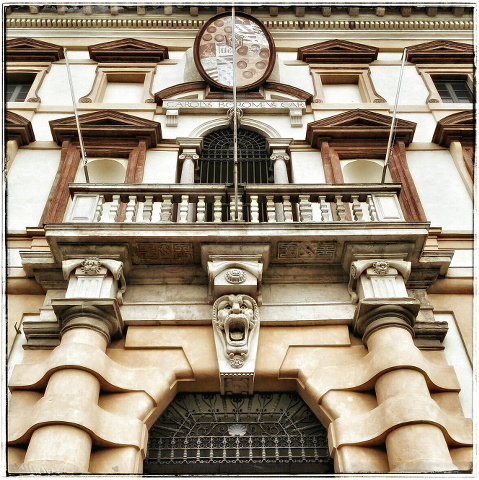
\includegraphics{smallthumb-lesson_I.jpeg}
\setfloatalignment{b}
\end{marginfigure}


\begin{abstract}
\noindent
Queste lezioni riprendono il testo introduttivo al Latino di Pearson\cite{pearson1915}, del quale seguono la numerazione; la struttura di ogni lezione è piuttosto regolare: inizia con \textsc{cenni di morfologia e di sintassi latina}, seguita da un \textsc{piccolo vocabolario} per il lessico; ci sono infine vari \textsc{esercizi} di traduzione e di composizione latina.

\bigskip
\noindent
Lezione II - Prima Declinazione, temi in -ā-, il caso Genitivo, il presente Indicativo di \textbf{sum}, interrogative, vocabolario, esercizi.
\end{abstract}

%\printclassoptions
% āēīōū
% ăĕĭŏŭ

\newthought{37. Frasi Modello.} Esamina le seguenti frasi:
 
\begin{itemize}
\item[\textsc{1.}] \textbf{Rosa puellae alba est}, \textit{la rosa della ragazza è bianca}.  
\item[\textsc{2.}] \textbf{Rosae puellarum albae sunt}, \textit{le rose delle ragazze sono bianche}.    
\end{itemize}
Osserva come \textbf{puellae} specifichi (limiti) \textbf{rosa}: non tutte le rose sono bianche, ma lo è quella quella della ragazza.
Allo stesso modo \textbf{puellarum} specifica \textbf{rosae}, perché definisce di quali rose si stia parlando.

\newthought{38. Regola di Sintassi.} Il caso Genitivo. Il genitivo è usato per specificare (limitare) o definire il significato di un nome.


\newthought{39. Verbo essere, modo Indicativo, tempo Presente}
\begin{fullwidth}
\begin{table}[!htbp]
  \centering
  \begin{tabular}{l l l}
    %\toprule
	\multicolumn{3}{c}{\textbf{sum}, \textit{io sono}}\\
	& \multicolumn{1}{c}{\textsc{Singolare}} & \multicolumn{1}{c}{\textsc{Plurale}}\\
	
    \textsc{1.} & \textbf{sum}, \textit{io sono} & \textbf{sumus}, \textit{noi siamo} \\
    \textsc{2.} & \textbf{es}, \textit{tu sei}   & \textbf{estis}, \textit{voi siete} \\
    \textsc{2.} & \textbf{est}, \textit{egli è}  & \textbf{sunt}, \textit{essi sono} \\
	
    %\bottomrule
  \end{tabular}
  %\caption[bottom]{Prima Declinazione. \textbf{stella, -ae}, f.}
  \label{tab:normaltab}
  %\zsavepos{pos:normaltab}
\end{table}
\end{fullwidth}


\newthought{40. Frasi Modello.} Esamina le seguenti frasi:
\\
\vspace{0.5em}
\noindent \textsc{Affermazione}\\
\noindent \hangindent=1em \textbf{Femina est pulchra}, \textit{la donna è bella}.
\\
\vspace{0.5em}
\noindent \textsc{Domande}
\begin{itemize}
\item[\textsc{1.}] \textbf{Estne femina pulchra?} \textit{è (quella) donna bella?} (risposta attesa, Sì o No).  
\item[\textsc{2.}] \textbf{Nonne femina pulchra est?}, \textit{non è bella (quella) donna?} (domanda retorica, la risposta attesa è Sì).    
\item[\textsc{3.}] \textbf{Ubi est femina?}, \textit{dov'è la donna?}    
\end{itemize}
Osserva \\
\begin{itemize}
\item[\textsc{1.}] Nelle domande semplici, alle quali si può rispondere con Sì o No, la particella enclitica \textbf{-ne} viene aggiunta alla parola enfatizzata, che di solito si trova a inizio frase. 
\item[\textsc{2.}] Le domande (retoriche) a cui ci si aspetta risposta affermativa, sono introdotte da \textbf{nonne}.  
\item[\textsc{3.}] Il \textbf{-ne} non si usa in domande introdotte da un pronome o avverbio interrogativo (\textbf{qui}, \textit{chi}, \textbf{ubi}, \textit{dove}, \textbf{cur}, \textit{perché}, ecc.).  
\end{itemize}

\newthought{41. Vocabolario}

\begin{multicols}{2}
    \noindent \hangindent=1em \textbf{pecunia, -ae}, f., \textit{moneta}.  \\
    \noindent \hangindent=1em \textbf{vita, -ae}, f., \textit{vita}.  \\
	\noindent \hangindent=1em \textbf{copia, -ae}, f., \textit{abbondanza} (al plurale \textbf{copiae, -arum}, \textit{truppe, forze}).  \\
	\noindent \hangindent=1em \textbf{femina, -ae}, f., \textit{donna}.  \\
	\noindent \hangindent=1em \textbf{patria, -ae}, f., \textit{patria, nazione}.  \\
	\noindent \hangindent=1em \textbf{Graecia, -ae}, f., \textit{Grecia}.  \\
	\noindent \hangindent=1em \textbf{Europa, -ae}, f., \textit{Europa}.  \\
	\noindent \hangindent=1em \textbf{Gallia, -ae}, f., \textit{Gallia}.  \\
	\noindent \hangindent=1em \textbf{filia, -ae}, f., \textit{figlia}.  \\

	\noindent \hangindent=1em \textbf{nova, -ae}, agg.f. \textit{nuova}.  \\
	\noindent \hangindent=1em \textbf{parva, -ae}, agg.f. \textit{piccola}.  \\
	\noindent \hangindent=1em \textbf{mea, -ae}, agg.f. \textit{mia}.  \\
	\noindent \hangindent=1em \textbf{tua, -ae}, agg.f. \textit{tua}.  \\
	
	\noindent \hangindent=1em \textbf{semper}, avv. \textit{sempre}.  \\
	
	\noindent \hangindent=1em \textbf{-ne}, enclitica, indica una domanda.  \\
	
\end{multicols}
% āēīōū
% ăĕĭŏŭ

\newthought{42. Esercizi}
\\
\textsc{I.} \quad
\textsc{1.}~Gallia est terra Europae. \quad
\textsc{2.}~Estne Gallia tua patria? \quad
\textsc{3.}~Nonne sunt parvae filiae? \quad
\textsc{4.}~Estne copia pecuniae? \quad
\textsc{5.}~Non longa est vita feminae. \quad
\textsc{6.}~Esi pulchra. \quad
\textsc{7.}~Copiae reginae non sunt magnae. \quad
\textsc{8.}~Suntne parvae puellae? \quad
\textsc{9.}~Regina tuae patriae pulchra est. \quad
\textsc{10.}~Copiae patriae meae non semper sunt parvae. \quad
\textsc{11.}~Reginarum rosae sunt pulchrae. \quad
\textsc{12.}~Semperne novae lunae pulchrae sunt? \quad
\textsc{13.}~Ubi sunt reginarum copiae? \quad
\textsc{14.}~Femiane Graeciae sunt pulchrae.
\\
\textsc{II.} \quad
\textsc{1.}~Noi siamo; tu sei; voi siete. \quad
\textsc{2.}~Dove siamo?. \quad
\textsc{3.}~Della bella donna. \quad
\textsc{4.}~Le truppe del mio paese sono poco numerose (trad. piccole). \quad
\textsc{5.}~Non c'è sempre abbondanza di monete. \quad
\textsc{6.}~Le figlie delle regine sono sempre belle? \quad
\textsc{7.}~Non è (forse) una bella nazione?

\newthought{(441). Lettura e Traduzione.} Un dialogo.
\\
Ubi est tua patria? Italia mea patria est; estne tua? Non est; mea patria Gallia est. Est terra Europae. 
Pulchrane Gallia est? Pulchra et lata terra est ubi longae viae sunt. Suntne silvae tuae patriae magnae?
Magnae non sunt, parva sunt. Nonne vita feminarum tuae patriae pulchra est? 
Feminarum bonarum vita semper pulchra et bona est.

\begin{figure}[!b]
  %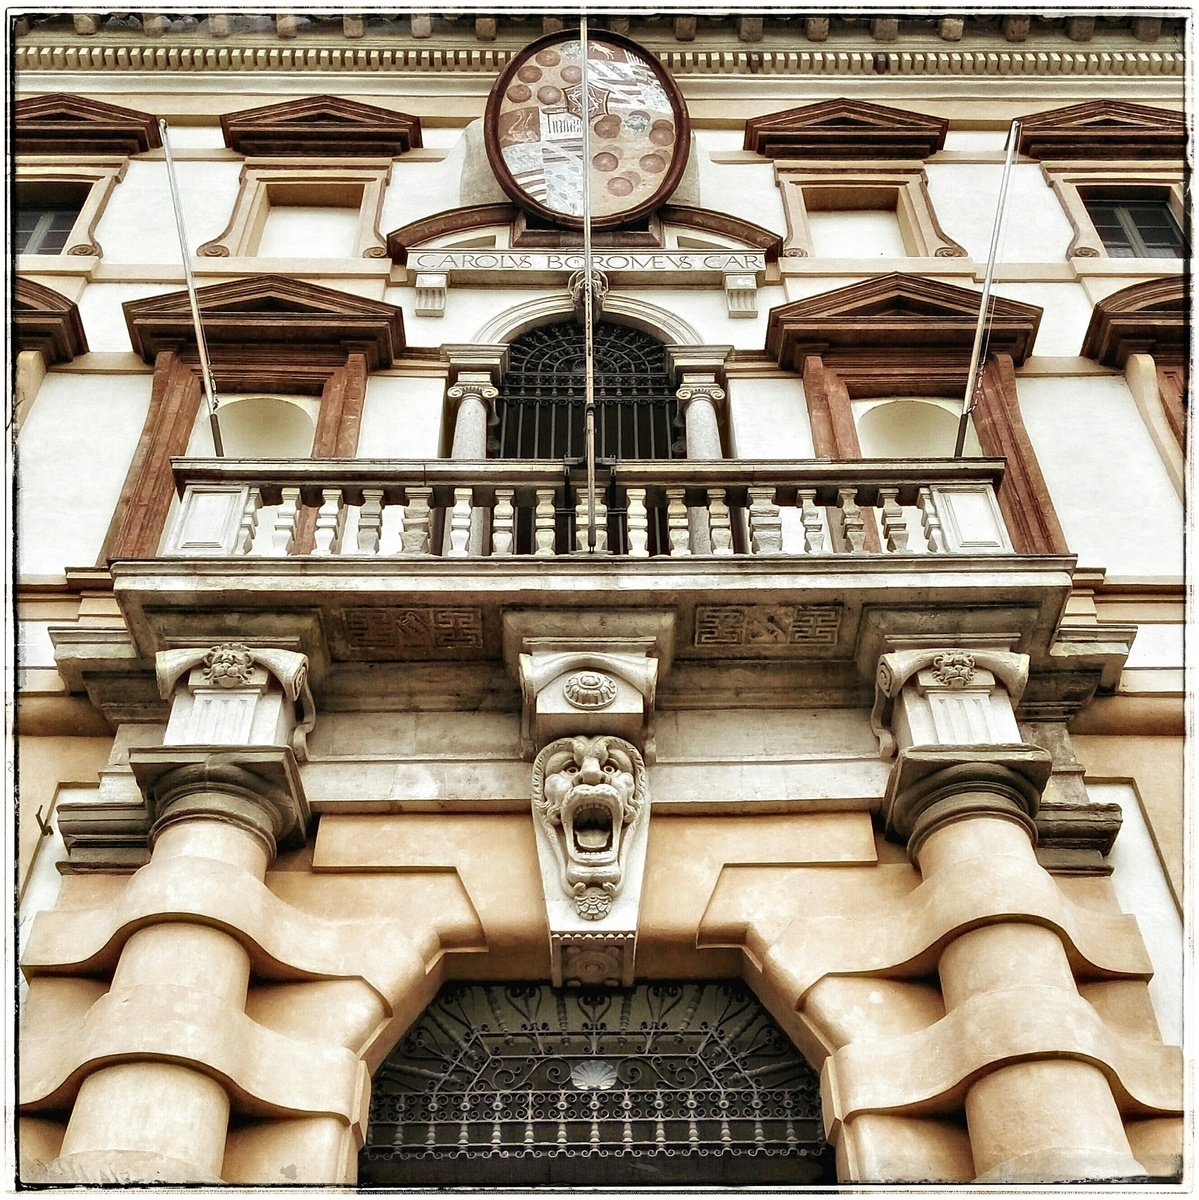
\includegraphics{thumb-lesson_I.jpeg}
  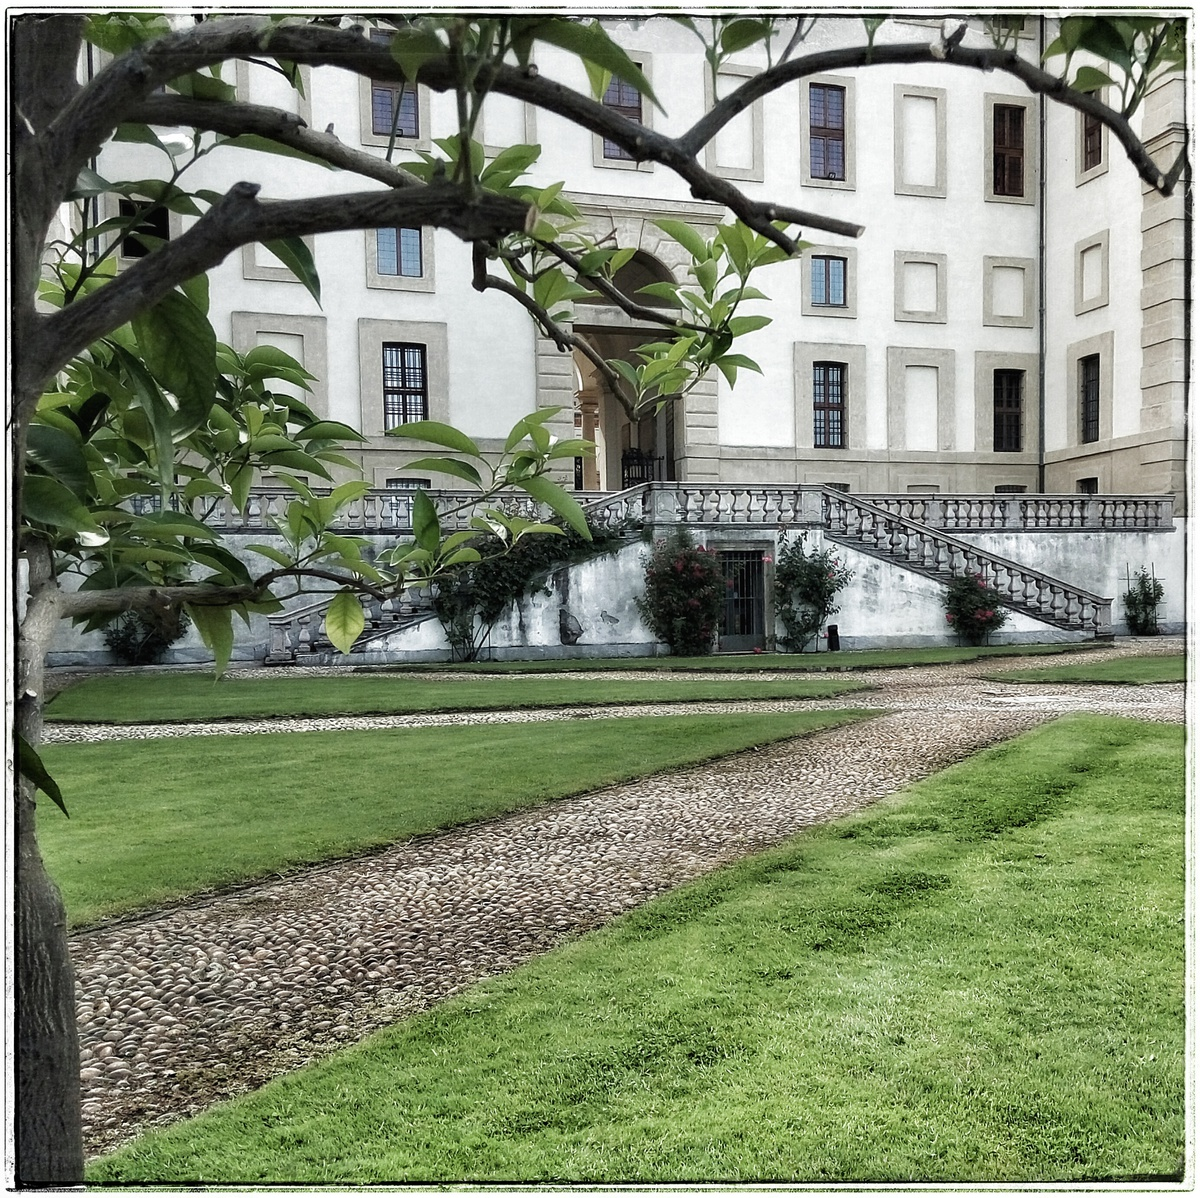
\includegraphics[width=0.8\linewidth]{thumb-lesson_III.jpeg}
  %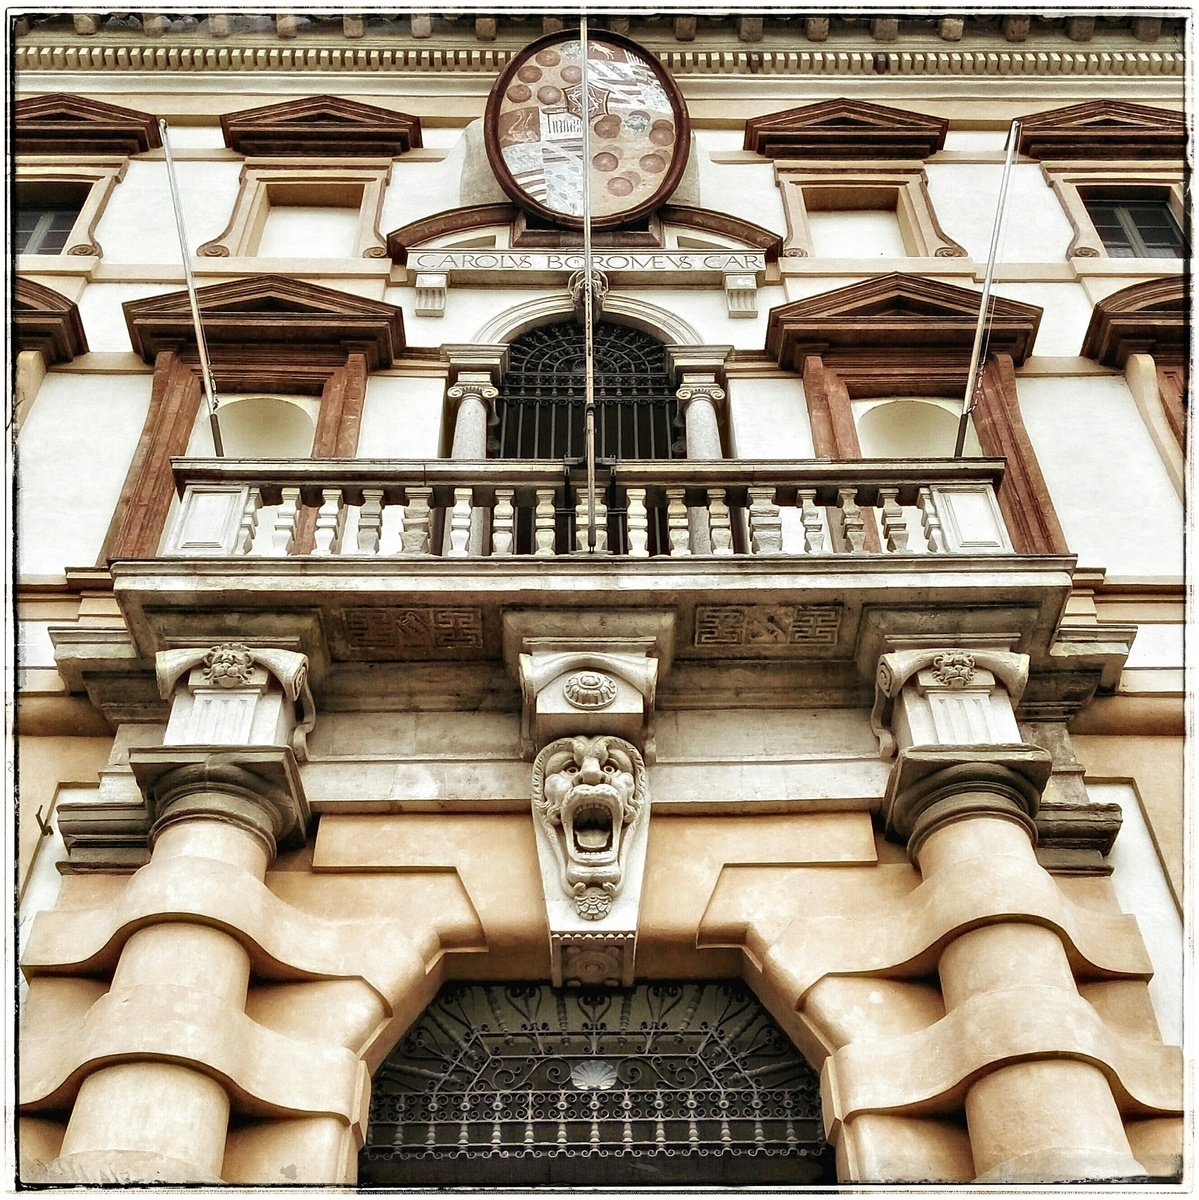
\includegraphics{thumb-lesson_I.jpeg}
  \caption{Pavia: Almo Collegio Borromeo}
  \label{fig:textfig}
  %\zsavepos{pos:textfig}
  %\setfloatalignment{b}
\end{figure}

 

\nobibliography{latinBiblio}
\bibliographystyle{alpha}


\end{document}
